\documentclass[1p]{elsarticle_modified}
%\bibliographystyle{elsarticle-num}

%\usepackage[colorlinks]{hyperref}
%\usepackage{abbrmath_seonhwa} %\Abb, \Ascr, \Acal ,\Abf, \Afrak
\usepackage{amsfonts}
\usepackage{amssymb}
\usepackage{amsmath}
\usepackage{amsthm}
\usepackage{scalefnt}
\usepackage{amsbsy}
\usepackage{kotex}
\usepackage{caption}
\usepackage{subfig}
\usepackage{color}
\usepackage{graphicx}
\usepackage{xcolor} %% white, black, red, green, blue, cyan, magenta, yellow
\usepackage{float}
\usepackage{setspace}
\usepackage{hyperref}

\usepackage{tikz}
\usetikzlibrary{arrows}

\usepackage{multirow}
\usepackage{array} % fixed length table
\usepackage{hhline}

%%%%%%%%%%%%%%%%%%%%%
\makeatletter
\renewcommand*\env@matrix[1][\arraystretch]{%
	\edef\arraystretch{#1}%
	\hskip -\arraycolsep
	\let\@ifnextchar\new@ifnextchar
	\array{*\c@MaxMatrixCols c}}
\makeatother %https://tex.stackexchange.com/questions/14071/how-can-i-increase-the-line-spacing-in-a-matrix
%%%%%%%%%%%%%%%

\usepackage[normalem]{ulem}

\newcommand{\msout}[1]{\ifmmode\text{\sout{\ensuremath{#1}}}\else\sout{#1}\fi}
%SOURCE: \msout is \stkout macro in https://tex.stackexchange.com/questions/20609/strikeout-in-math-mode

\newcommand{\cancel}[1]{
	\ifmmode
	{\color{red}\msout{#1}}
	\else
	{\color{red}\sout{#1}}
	\fi
}

\newcommand{\add}[1]{
	{\color{blue}\uwave{#1}}
}

\newcommand{\replace}[2]{
	\ifmmode
	{\color{red}\msout{#1}}{\color{blue}\uwave{#2}}
	\else
	{\color{red}\sout{#1}}{\color{blue}\uwave{#2}}
	\fi
}

\newcommand{\Sol}{\mathcal{S}} %segment
\newcommand{\D}{D} %diagram
\newcommand{\A}{\mathcal{A}} %arc


%%%%%%%%%%%%%%%%%%%%%%%%%%%%%5 test

\def\sl{\operatorname{\textup{SL}}(2,\Cbb)}
\def\psl{\operatorname{\textup{PSL}}(2,\Cbb)}
\def\quan{\mkern 1mu \triangleright \mkern 1mu}

\theoremstyle{definition}
\newtheorem{thm}{Theorem}[section]
\newtheorem{prop}[thm]{Proposition}
\newtheorem{lem}[thm]{Lemma}
\newtheorem{ques}[thm]{Question}
\newtheorem{cor}[thm]{Corollary}
\newtheorem{defn}[thm]{Definition}
\newtheorem{exam}[thm]{Example}
\newtheorem{rmk}[thm]{Remark}
\newtheorem{alg}[thm]{Algorithm}

\newcommand{\I}{\sqrt{-1}}
\begin{document}

%\begin{frontmatter}
%
%\title{Boundary parabolic representations of knots up to 8 crossings}
%
%%% Group authors per affiliation:
%\author{Yunhi Cho} 
%\address{Department of Mathematics, University of Seoul, Seoul, Korea}
%\ead{yhcho@uos.ac.kr}
%
%
%\author{Seonhwa Kim} %\fnref{s_kim}}
%\address{Center for Geometry and Physics, Institute for Basic Science, Pohang, 37673, Korea}
%\ead{ryeona17@ibs.re.kr}
%
%\author{Hyuk Kim}
%\address{Department of Mathematical Sciences, Seoul National University, Seoul 08826, Korea}
%\ead{hyukkim@snu.ac.kr}
%
%\author{Seokbeom Yoon}
%\address{Department of Mathematical Sciences, Seoul National University, Seoul, 08826,  Korea}
%\ead{sbyoon15@snu.ac.kr}
%
%\begin{abstract}
%We find all boundary parabolic representation of knots up to 8 crossings.
%
%\end{abstract}
%\begin{keyword}
%    \MSC[2010] 57M25 
%\end{keyword}
%
%\end{frontmatter}

%\linenumbers
%\tableofcontents
%
\newcommand\colored[1]{\textcolor{white}{\rule[-0.35ex]{0.8em}{1.4ex}}\kern-0.8em\color{red} #1}%
%\newcommand\colored[1]{\textcolor{white}{ #1}\kern-2.17ex	\textcolor{white}{ #1}\kern-1.81ex	\textcolor{white}{ #1}\kern-2.15ex\color{red}#1	}

{\Large $\underline{12a_{0742}~(K12a_{0742})}$}

\setlength{\tabcolsep}{10pt}
\renewcommand{\arraystretch}{1.6}
\vspace{1cm}\begin{tabular}{m{100pt}>{\centering\arraybackslash}m{274pt}}
\multirow{5}{120pt}{
	\centering
	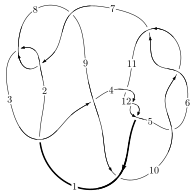
\includegraphics[width=112pt]{../../../GIT/diagram.site/Diagrams/png/1543_12a_0742.png}\\
\ \ \ A knot diagram\footnotemark}&
\allowdisplaybreaks
\textbf{Linearized knot diagam} \\
\cline{2-2}
 &
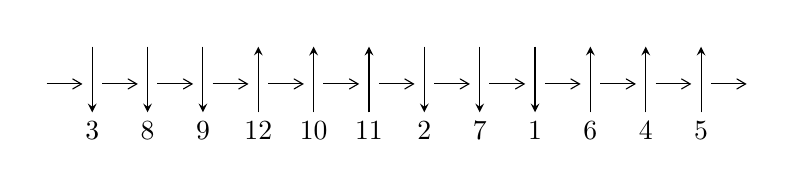
\begin{tikzpicture}[x=20pt, y=17pt]
	% nodes
	\node (C0) at (0, 0) {};
	\node (C1) at (1, 0) {};
	\node (C1U) at (1, +1) {};
	\node (C1D) at (1, -1) {3};

	\node (C2) at (2, 0) {};
	\node (C2U) at (2, +1) {};
	\node (C2D) at (2, -1) {8};

	\node (C3) at (3, 0) {};
	\node (C3U) at (3, +1) {};
	\node (C3D) at (3, -1) {9};

	\node (C4) at (4, 0) {};
	\node (C4U) at (4, +1) {};
	\node (C4D) at (4, -1) {12};

	\node (C5) at (5, 0) {};
	\node (C5U) at (5, +1) {};
	\node (C5D) at (5, -1) {10};

	\node (C6) at (6, 0) {};
	\node (C6U) at (6, +1) {};
	\node (C6D) at (6, -1) {11};

	\node (C7) at (7, 0) {};
	\node (C7U) at (7, +1) {};
	\node (C7D) at (7, -1) {2};

	\node (C8) at (8, 0) {};
	\node (C8U) at (8, +1) {};
	\node (C8D) at (8, -1) {7};

	\node (C9) at (9, 0) {};
	\node (C9U) at (9, +1) {};
	\node (C9D) at (9, -1) {1};

	\node (C10) at (10, 0) {};
	\node (C10U) at (10, +1) {};
	\node (C10D) at (10, -1) {6};

	\node (C11) at (11, 0) {};
	\node (C11U) at (11, +1) {};
	\node (C11D) at (11, -1) {4};

	\node (C12) at (12, 0) {};
	\node (C12U) at (12, +1) {};
	\node (C12D) at (12, -1) {5};
	\node (C13) at (13, 0) {};

	% arrows
	\draw[->,>={angle 60}]
	(C0) edge (C1) (C1) edge (C2) (C2) edge (C3) (C3) edge (C4) (C4) edge (C5) (C5) edge (C6) (C6) edge (C7) (C7) edge (C8) (C8) edge (C9) (C9) edge (C10) (C10) edge (C11) (C11) edge (C12) (C12) edge (C13) ;	\draw[->,>=stealth]
	(C1U) edge (C1D) (C2U) edge (C2D) (C3U) edge (C3D) (C4D) edge (C4U) (C5D) edge (C5U) (C6D) edge (C6U) (C7U) edge (C7D) (C8U) edge (C8D) (C9U) edge (C9D) (C10D) edge (C10U) (C11D) edge (C11U) (C12D) edge (C12U) ;
	\end{tikzpicture} \\
\hhline{~~} \\& 
\textbf{Solving Sequence} \\ \cline{2-2} 
 &
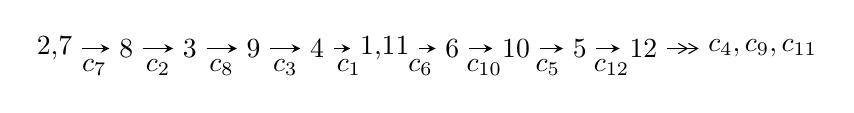
\begin{tikzpicture}[x=23pt, y=7pt]
	% node
	\node (A0) at (-1/8, 0) {2,7};
	\node (A1) at (1, 0) {8};
	\node (A2) at (2, 0) {3};
	\node (A3) at (3, 0) {9};
	\node (A4) at (4, 0) {4};
	\node (A5) at (81/16, 0) {1,11};
	\node (A6) at (49/8, 0) {6};
	\node (A7) at (57/8, 0) {10};
	\node (A8) at (65/8, 0) {5};
	\node (A9) at (73/8, 0) {12};
	\node (C1) at (1/2, -1) {$c_{7}$};
	\node (C2) at (3/2, -1) {$c_{2}$};
	\node (C3) at (5/2, -1) {$c_{8}$};
	\node (C4) at (7/2, -1) {$c_{3}$};
	\node (C5) at (9/2, -1) {$c_{1}$};
	\node (C6) at (45/8, -1) {$c_{6}$};
	\node (C7) at (53/8, -1) {$c_{10}$};
	\node (C8) at (61/8, -1) {$c_{5}$};
	\node (C9) at (69/8, -1) {$c_{12}$};
	\node (A10) at (11, 0) {$c_{4},c_{9},c_{11}$};

	% edge
	\draw[->,>=stealth]	
	(A0) edge (A1) (A1) edge (A2) (A2) edge (A3) (A3) edge (A4) (A4) edge (A5) (A5) edge (A6) (A6) edge (A7) (A7) edge (A8) (A8) edge (A9) ;
	\draw[->>,>={angle 60}]	
	(A9) edge (A10);
\end{tikzpicture} \\ 

\end{tabular} \\

\footnotetext{
The image of knot diagram is generated by the software ``\textbf{Draw programme}" developed by Andrew Bartholomew(\url{http://www.layer8.co.uk/maths/draw/index.htm\#Running-draw}), where we modified some parts for our purpose(\url{https://github.com/CATsTAILs/LinksPainter}).
}\phantom \\ \newline 
\centering \textbf{Ideals for irreducible components\footnotemark of $X_{\text{par}}$} 
 
\begin{align*}
I^u_{1}&=\langle 
u^{32}- u^{31}+\cdots+b-1,\;- u^{33}+5 u^{32}+\cdots+2 a-8,\;u^{34}-3 u^{33}+\cdots+8 u-2\rangle \\
I^u_{2}&=\langle 
-2 u^4 a- u^3 a+3 u^4+u^3- u^2+2 b-3 a+6,\;-2 u^4 a- u^3 a+3 u^4+3 u^3+a^2+a u-2 u^2-3 a+u+4,\\
\phantom{I^u_{2}}&\phantom{= \langle  }u^5+u^4+2 u+1\rangle \\
I^u_{3}&=\langle 
b-1,\;u^3+2 u^2+2 a- u,\;u^4- u^2+2\rangle \\
I^u_{4}&=\langle 
-3 u^{15} a-4 u^{14} a+\cdots-6 a+4,\;u^{15} a- u^{15}+\cdots+a^2- a,\\
\phantom{I^u_{4}}&\phantom{= \langle  }u^{16}+u^{15}-2 u^{14}-3 u^{13}+4 u^{12}+7 u^{11}-3 u^{10}-10 u^9+9 u^7+3 u^6-5 u^5-4 u^4+2 u^2+2 u+1\rangle \\
I^u_{5}&=\langle 
b+1,\;a+u-1,\;u^4+1\rangle \\
I^u_{6}&=\langle 
b,\;a+1,\;u-1\rangle \\
I^u_{7}&=\langle 
b-1,\;a-1,\;u-1\rangle \\
I^u_{8}&=\langle 
b-1,\;a,\;u-1\rangle \\
I^u_{9}&=\langle 
b-1,\;a-2,\;u+1\rangle \\
\\
I^v_{1}&=\langle 
a,\;b+1,\;v+1\rangle \\
\end{align*}
\raggedright * 10 irreducible components of $\dim_{\mathbb{C}}=0$, with total 89 representations.\\
\footnotetext{All coefficients of polynomials are rational numbers. But the coefficients are sometimes approximated in decimal forms when there is not enough margin.}
\newpage
\renewcommand{\arraystretch}{1}
\centering \section*{I. $I^u_{1}= \langle u^{32}- u^{31}+\cdots+b-1,\;- u^{33}+5 u^{32}+\cdots+2 a-8,\;u^{34}-3 u^{33}+\cdots+8 u-2 \rangle$}
\flushleft \textbf{(i) Arc colorings}\\
\begin{tabular}{m{7pt} m{180pt} m{7pt} m{180pt} }
\flushright $a_{2}=$&$\begin{pmatrix}0\\u\end{pmatrix}$ \\
\flushright $a_{7}=$&$\begin{pmatrix}1\\0\end{pmatrix}$ \\
\flushright $a_{8}=$&$\begin{pmatrix}1\\u^2\end{pmatrix}$ \\
\flushright $a_{3}=$&$\begin{pmatrix}- u\\- u^3+u\end{pmatrix}$ \\
\flushright $a_{9}=$&$\begin{pmatrix}- u^2+1\\u^2\end{pmatrix}$ \\
\flushright $a_{4}=$&$\begin{pmatrix}u^7-2 u^5+2 u^3-2 u\\- u^7+u^5-2 u^3+u\end{pmatrix}$ \\
\flushright $a_{1}=$&$\begin{pmatrix}u^3\\u^5- u^3+u\end{pmatrix}$ \\
\flushright $a_{11}=$&$\begin{pmatrix}\frac{1}{2} u^{33}-\frac{5}{2} u^{32}+\cdots-9 u+4\\- u^{32}+u^{31}+\cdots-4 u+1\end{pmatrix}$ \\
\flushright $a_{6}=$&$\begin{pmatrix}\frac{3}{2} u^{33}-\frac{7}{2} u^{32}+\cdots-8 u+3\\- u^{33}+2 u^{32}+\cdots+4 u-1\end{pmatrix}$ \\
\flushright $a_{10}=$&$\begin{pmatrix}- u^{10}+u^8-2 u^6+u^4- u^2+1\\- u^{12}+2 u^{10}-4 u^8+4 u^6-3 u^4+2 u^2\end{pmatrix}$ \\
\flushright $a_{5}=$&$\begin{pmatrix}\frac{7}{2} u^{33}-\frac{17}{2} u^{32}+\cdots-20 u+6\\-3 u^{33}+6 u^{32}+\cdots+12 u-3\end{pmatrix}$ \\
\flushright $a_{12}=$&$\begin{pmatrix}\frac{1}{2} u^{33}-\frac{3}{2} u^{32}+\cdots-5 u+2\\- u^{32}+u^{31}+\cdots-3 u+1\end{pmatrix}$\\&\end{tabular}
\flushleft \textbf{(ii) Obstruction class $= -1$}\\~\\
\flushleft \textbf{(iii) Cusp Shapes $= -8 u^{33}+18 u^{32}+24 u^{31}-98 u^{30}-34 u^{29}+324 u^{28}-48 u^{27}-778 u^{26}+404 u^{25}+1380 u^{24}-1192 u^{23}-1882 u^{22}+2412 u^{21}+1850 u^{20}-3712 u^{19}-984 u^{18}+4390 u^{17}-460 u^{16}-3998 u^{15}+1854 u^{14}+2552 u^{13}-2452 u^{12}-726 u^{11}+1942 u^{10}-470 u^9-954 u^8+796 u^7+110 u^6-512 u^5+270 u^4+50 u^3-132 u^2+74 u-20$}\\~\\
\newpage\renewcommand{\arraystretch}{1}
\flushleft \textbf{(iv) u-Polynomials at the component}\newline \\
\begin{tabular}{m{50pt}|m{274pt}}
Crossings & \hspace{64pt}u-Polynomials at each crossing \\
\hline $$\begin{aligned}c_{1},c_{8}\end{aligned}$$&$\begin{aligned}
&u^{34}+11 u^{33}+\cdots-16 u+4
\end{aligned}$\\
\hline $$\begin{aligned}c_{2},c_{7}\end{aligned}$$&$\begin{aligned}
&u^{34}+3 u^{33}+\cdots-8 u-2
\end{aligned}$\\
\hline $$\begin{aligned}c_{3}\end{aligned}$$&$\begin{aligned}
&u^{34}-3 u^{33}+\cdots+848 u-296
\end{aligned}$\\
\hline $$\begin{aligned}c_{4},c_{5},c_{6}\\c_{10},c_{11},c_{12}\end{aligned}$$&$\begin{aligned}
&u^{34}- u^{33}+\cdots+u+1
\end{aligned}$\\
\hline $$\begin{aligned}c_{9}\end{aligned}$$&$\begin{aligned}
&u^{34}+21 u^{33}+\cdots-40228 u-4366
\end{aligned}$\\
\hline
\end{tabular}\\~\\
\newpage\renewcommand{\arraystretch}{1}
\flushleft \textbf{(v) Riley Polynomials at the component}\newline \\
\begin{tabular}{m{50pt}|m{274pt}}
Crossings & \hspace{64pt}Riley Polynomials at each crossing \\
\hline $$\begin{aligned}c_{1},c_{8}\end{aligned}$$&$\begin{aligned}
&y^{34}+25 y^{33}+\cdots-288 y+16
\end{aligned}$\\
\hline $$\begin{aligned}c_{2},c_{7}\end{aligned}$$&$\begin{aligned}
&y^{34}-11 y^{33}+\cdots+16 y+4
\end{aligned}$\\
\hline $$\begin{aligned}c_{3}\end{aligned}$$&$\begin{aligned}
&y^{34}+y^{33}+\cdots+674464 y+87616
\end{aligned}$\\
\hline $$\begin{aligned}c_{4},c_{5},c_{6}\\c_{10},c_{11},c_{12}\end{aligned}$$&$\begin{aligned}
&y^{34}-43 y^{33}+\cdots-9 y+1
\end{aligned}$\\
\hline $$\begin{aligned}c_{9}\end{aligned}$$&$\begin{aligned}
&y^{34}+13 y^{33}+\cdots+56365904 y+19061956
\end{aligned}$\\
\hline
\end{tabular}\\~\\
\newpage\flushleft \textbf{(vi) Complex Volumes and Cusp Shapes}
$$\begin{array}{c|c|c}  
\text{Solutions to }I^u_{1}& \I (\text{vol} + \sqrt{-1}CS) & \text{Cusp shape}\\
 \hline 
\begin{aligned}
u &= -0.988927 + 0.109578 I \\
a &= -0.431526 + 1.228470 I \\
b &= \phantom{-}0.276236 + 0.567180 I\end{aligned}
 & -3.24927 + 2.65062 I & -6.82528 - 6.63039 I \\ \hline\begin{aligned}
u &= -0.988927 - 0.109578 I \\
a &= -0.431526 - 1.228470 I \\
b &= \phantom{-}0.276236 - 0.567180 I\end{aligned}
 & -3.24927 - 2.65062 I & -6.82528 + 6.63039 I \\ \hline\begin{aligned}
u &= -0.739127 + 0.741106 I \\
a &= \phantom{-}0.930370 + 0.017261 I \\
b &= -0.485252 - 0.215051 I\end{aligned}
 & \phantom{-}3.09736 + 0.68740 I & \phantom{-}3.83595 - 3.91295 I \\ \hline\begin{aligned}
u &= -0.739127 - 0.741106 I \\
a &= \phantom{-}0.930370 - 0.017261 I \\
b &= -0.485252 + 0.215051 I\end{aligned}
 & \phantom{-}3.09736 - 0.68740 I & \phantom{-}3.83595 + 3.91295 I \\ \hline\begin{aligned}
u &= \phantom{-}0.718436 + 0.774498 I \\
a &= \phantom{-}0.812978 + 0.075813 I \\
b &= -0.412168 - 0.529259 I\end{aligned}
 & \phantom{-}2.64462 + 2.18332 I & \phantom{-}2.21430 - 4.77335 I \\ \hline\begin{aligned}
u &= \phantom{-}0.718436 - 0.774498 I \\
a &= \phantom{-}0.812978 - 0.075813 I \\
b &= -0.412168 + 0.529259 I\end{aligned}
 & \phantom{-}2.64462 - 2.18332 I & \phantom{-}2.21430 + 4.77335 I \\ \hline\begin{aligned}
u &= \phantom{-}0.939426\phantom{ +0.000000I} \\
a &= \phantom{-}0.0259566\phantom{ +0.000000I} \\
b &= \phantom{-}0.428300\phantom{ +0.000000I}\end{aligned}
 & -1.90429\phantom{ +0.000000I} & -3.14100\phantom{ +0.000000I} \\ \hline\begin{aligned}
u &= \phantom{-}0.891331 + 0.603370 I \\
a &= \phantom{-}0.422005 + 0.483472 I \\
b &= \phantom{-}0.066256 + 0.592921 I\end{aligned}
 & -0.69654 - 2.34709 I & -4.49475 + 2.27928 I \\ \hline\begin{aligned}
u &= \phantom{-}0.891331 - 0.603370 I \\
a &= \phantom{-}0.422005 - 0.483472 I \\
b &= \phantom{-}0.066256 - 0.592921 I\end{aligned}
 & -0.69654 + 2.34709 I & -4.49475 - 2.27928 I \\ \hline\begin{aligned}
u &= \phantom{-}1.005180 + 0.389797 I \\
a &= -0.154937 + 0.640657 I \\
b &= -1.52677 - 0.22591 I\end{aligned}
 & \phantom{-}9.88665 + 2.86032 I & \phantom{-}4.26747 + 0.39615 I\\
 \hline 
 \end{array}$$\newpage$$\begin{array}{c|c|c}  
\text{Solutions to }I^u_{1}& \I (\text{vol} + \sqrt{-1}CS) & \text{Cusp shape}\\
 \hline 
\begin{aligned}
u &= \phantom{-}1.005180 - 0.389797 I \\
a &= -0.154937 - 0.640657 I \\
b &= -1.52677 + 0.22591 I\end{aligned}
 & \phantom{-}9.88665 - 2.86032 I & \phantom{-}4.26747 - 0.39615 I \\ \hline\begin{aligned}
u &= -1.076760 + 0.192034 I \\
a &= -0.23388 - 1.88626 I \\
b &= -1.52621 - 0.30047 I\end{aligned}
 & \phantom{-}8.67508 + 9.43470 I & \phantom{-}2.55855 - 6.18677 I \\ \hline\begin{aligned}
u &= -1.076760 - 0.192034 I \\
a &= -0.23388 + 1.88626 I \\
b &= -1.52621 + 0.30047 I\end{aligned}
 & \phantom{-}8.67508 - 9.43470 I & \phantom{-}2.55855 + 6.18677 I \\ \hline\begin{aligned}
u &= -1.10214\phantom{ +0.000000I} \\
a &= \phantom{-}1.33391\phantom{ +0.000000I} \\
b &= \phantom{-}1.42323\phantom{ +0.000000I}\end{aligned}
 & \phantom{-}3.37001\phantom{ +0.000000I} & \phantom{-}2.15130\phantom{ +0.000000I} \\ \hline\begin{aligned}
u &= \phantom{-}0.701066 + 0.850551 I \\
a &= -2.07986 + 0.41696 I \\
b &= \phantom{-}1.56353 + 0.32987 I\end{aligned}
 & \phantom{-}15.6899 + 9.3353 I & \phantom{-}8.75460 - 3.54458 I \\ \hline\begin{aligned}
u &= \phantom{-}0.701066 - 0.850551 I \\
a &= -2.07986 - 0.41696 I \\
b &= \phantom{-}1.56353 - 0.32987 I\end{aligned}
 & \phantom{-}15.6899 - 9.3353 I & \phantom{-}8.75460 + 3.54458 I \\ \hline\begin{aligned}
u &= \phantom{-}0.506457 + 0.733877 I \\
a &= \phantom{-}1.048590 + 0.101195 I \\
b &= -1.46790 - 0.05121 I\end{aligned}
 & \phantom{-}8.81248 + 1.35417 I & \phantom{-}8.27726 - 0.26965 I \\ \hline\begin{aligned}
u &= \phantom{-}0.506457 - 0.733877 I \\
a &= \phantom{-}1.048590 - 0.101195 I \\
b &= -1.46790 + 0.05121 I\end{aligned}
 & \phantom{-}8.81248 - 1.35417 I & \phantom{-}8.27726 + 0.26965 I \\ \hline\begin{aligned}
u &= -0.804999 + 0.836403 I \\
a &= -2.48607 + 0.64116 I \\
b &= \phantom{-}1.62501 + 0.21278 I\end{aligned}
 & \phantom{-}17.5746 + 4.9413 I & \phantom{-}9.92383 - 3.25429 I \\ \hline\begin{aligned}
u &= -0.804999 - 0.836403 I \\
a &= -2.48607 - 0.64116 I \\
b &= \phantom{-}1.62501 - 0.21278 I\end{aligned}
 & \phantom{-}17.5746 - 4.9413 I & \phantom{-}9.92383 + 3.25429 I\\
 \hline 
 \end{array}$$\newpage$$\begin{array}{c|c|c}  
\text{Solutions to }I^u_{1}& \I (\text{vol} + \sqrt{-1}CS) & \text{Cusp shape}\\
 \hline 
\begin{aligned}
u &= -0.966971 + 0.696899 I \\
a &= -0.486334 + 0.622660 I \\
b &= \phantom{-}0.511243 - 0.168909 I\end{aligned}
 & \phantom{-}2.40071 + 4.80114 I & \phantom{-}1.91928 - 2.14166 I \\ \hline\begin{aligned}
u &= -0.966971 - 0.696899 I \\
a &= -0.486334 - 0.622660 I \\
b &= \phantom{-}0.511243 + 0.168909 I\end{aligned}
 & \phantom{-}2.40071 - 4.80114 I & \phantom{-}1.91928 + 2.14166 I \\ \hline\begin{aligned}
u &= \phantom{-}1.032170 + 0.632265 I \\
a &= -0.17093 - 1.70332 I \\
b &= \phantom{-}1.43085 - 0.07072 I\end{aligned}
 & \phantom{-}7.31130 - 6.52330 I & \phantom{-}5.94001 + 5.49172 I \\ \hline\begin{aligned}
u &= \phantom{-}1.032170 - 0.632265 I \\
a &= -0.17093 + 1.70332 I \\
b &= \phantom{-}1.43085 + 0.07072 I\end{aligned}
 & \phantom{-}7.31130 + 6.52330 I & \phantom{-}5.94001 - 5.49172 I \\ \hline\begin{aligned}
u &= \phantom{-}0.986491 + 0.714526 I \\
a &= -1.35111 - 0.66802 I \\
b &= \phantom{-}0.407979 - 0.571160 I\end{aligned}
 & \phantom{-}1.83243 - 7.82430 I & \phantom{-}0.40818 + 9.67142 I \\ \hline\begin{aligned}
u &= \phantom{-}0.986491 - 0.714526 I \\
a &= -1.35111 + 0.66802 I \\
b &= \phantom{-}0.407979 + 0.571160 I\end{aligned}
 & \phantom{-}1.83243 + 7.82430 I & \phantom{-}0.40818 - 9.67142 I \\ \hline\begin{aligned}
u &= -0.957491 + 0.784549 I \\
a &= \phantom{-}1.91646 - 1.35507 I \\
b &= -1.62922 + 0.19094 I\end{aligned}
 & \phantom{-}17.1033 + 1.1035 I & \phantom{-}9.17994 - 1.90960 I \\ \hline\begin{aligned}
u &= -0.957491 - 0.784549 I \\
a &= \phantom{-}1.91646 + 1.35507 I \\
b &= -1.62922 - 0.19094 I\end{aligned}
 & \phantom{-}17.1033 - 1.1035 I & \phantom{-}9.17994 + 1.90960 I \\ \hline\begin{aligned}
u &= \phantom{-}1.022640 + 0.743834 I \\
a &= \phantom{-}1.85346 + 2.37415 I \\
b &= -1.55431 + 0.34115 I\end{aligned}
 & \phantom{-}14.7022 - 15.2836 I & \phantom{-}7.11885 + 8.33563 I \\ \hline\begin{aligned}
u &= \phantom{-}1.022640 - 0.743834 I \\
a &= \phantom{-}1.85346 - 2.37415 I \\
b &= -1.55431 - 0.34115 I\end{aligned}
 & \phantom{-}14.7022 + 15.2836 I & \phantom{-}7.11885 - 8.33563 I\\
 \hline 
 \end{array}$$\newpage$$\begin{array}{c|c|c}  
\text{Solutions to }I^u_{1}& \I (\text{vol} + \sqrt{-1}CS) & \text{Cusp shape}\\
 \hline 
\begin{aligned}
u &= \phantom{-}0.122815 + 0.705145 I \\
a &= -2.12345 - 0.61721 I \\
b &= \phantom{-}1.55687 - 0.26874 I\end{aligned}
 & \phantom{-}12.6181 - 6.5965 I & \phantom{-}9.17145 + 3.77893 I \\ \hline\begin{aligned}
u &= \phantom{-}0.122815 - 0.705145 I \\
a &= -2.12345 + 0.61721 I \\
b &= \phantom{-}1.55687 + 0.26874 I\end{aligned}
 & \phantom{-}12.6181 + 6.5965 I & \phantom{-}9.17145 - 3.77893 I \\ \hline\begin{aligned}
u &= \phantom{-}0.129052 + 0.423858 I \\
a &= \phantom{-}0.854310 + 0.046698 I \\
b &= -0.261902 + 0.382447 I\end{aligned}
 & \phantom{-}0.121984 - 0.976428 I & \phantom{-}2.24524 + 6.97728 I \\ \hline\begin{aligned}
u &= \phantom{-}0.129052 - 0.423858 I \\
a &= \phantom{-}0.854310 - 0.046698 I \\
b &= -0.261902 - 0.382447 I\end{aligned}
 & \phantom{-}0.121984 + 0.976428 I & \phantom{-}2.24524 - 6.97728 I\\
 \hline 
 \end{array}$$\newpage\newpage\renewcommand{\arraystretch}{1}
\centering \section*{II. $I^u_{2}= \langle -2 u^4 a- u^3 a+3 u^4+u^3- u^2+2 b-3 a+6,\;-2 u^4 a+3 u^4+\cdots-3 a+4,\;u^5+u^4+2 u+1 \rangle$}
\flushleft \textbf{(i) Arc colorings}\\
\begin{tabular}{m{7pt} m{180pt} m{7pt} m{180pt} }
\flushright $a_{2}=$&$\begin{pmatrix}0\\u\end{pmatrix}$ \\
\flushright $a_{7}=$&$\begin{pmatrix}1\\0\end{pmatrix}$ \\
\flushright $a_{8}=$&$\begin{pmatrix}1\\u^2\end{pmatrix}$ \\
\flushright $a_{3}=$&$\begin{pmatrix}- u\\- u^3+u\end{pmatrix}$ \\
\flushright $a_{9}=$&$\begin{pmatrix}- u^2+1\\u^2\end{pmatrix}$ \\
\flushright $a_{4}=$&$\begin{pmatrix}u^4+u^2+u+1\\- u^2\end{pmatrix}$ \\
\flushright $a_{1}=$&$\begin{pmatrix}u^3\\- u^4- u^3- u-1\end{pmatrix}$ \\
\flushright $a_{11}=$&$\begin{pmatrix}a\\u^4 a-\frac{3}{2} u^4+\cdots+\frac{3}{2} a-3\end{pmatrix}$ \\
\flushright $a_{6}=$&$\begin{pmatrix}\frac{3}{2} u^4 a- u^4+\cdots+3 a-3\\-\frac{1}{2} u^4 a+u^4+\cdots- a+\frac{5}{2}\end{pmatrix}$ \\
\flushright $a_{10}=$&$\begin{pmatrix}u^4- u^2+2 u+2\\u^3- u\end{pmatrix}$ \\
\flushright $a_{5}=$&$\begin{pmatrix}2 u^4 a-2 u^4+\cdots+4 a-\frac{11}{2}\\-\frac{1}{2} u^4 a+\frac{1}{2} u^4+\cdots-\frac{1}{2} a+\frac{3}{2}\end{pmatrix}$ \\
\flushright $a_{12}=$&$\begin{pmatrix}u^4 a-\frac{1}{2} u^4+\cdots+\frac{5}{2} a-2\\\frac{1}{2} u^4 a- u^4+\cdots+a-2\end{pmatrix}$\\&\end{tabular}
\flushleft \textbf{(ii) Obstruction class $= -1$}\\~\\
\flushleft \textbf{(iii) Cusp Shapes $= -4 u^4-4 u^3+4 u^2-2$}\\~\\
\newpage\renewcommand{\arraystretch}{1}
\flushleft \textbf{(iv) u-Polynomials at the component}\newline \\
\begin{tabular}{m{50pt}|m{274pt}}
Crossings & \hspace{64pt}u-Polynomials at each crossing \\
\hline $$\begin{aligned}c_{1},c_{8}\end{aligned}$$&$\begin{aligned}
&(u^5+u^4+4 u^3+2 u^2+4 u+1)^2
\end{aligned}$\\
\hline $$\begin{aligned}c_{2},c_{7}\end{aligned}$$&$\begin{aligned}
&(u^5- u^4+2 u-1)^2
\end{aligned}$\\
\hline $$\begin{aligned}c_{3}\end{aligned}$$&$\begin{aligned}
&(u^5+4 u^4+9 u^3+9 u^2+4 u-4)^2
\end{aligned}$\\
\hline $$\begin{aligned}c_{4},c_{5},c_{6}\\c_{10},c_{11},c_{12}\end{aligned}$$&$\begin{aligned}
&u^{10}- u^9-4 u^8+4 u^7+4 u^6-3 u^5-3 u^4- u^3+9 u^2-2 u-5
\end{aligned}$\\
\hline $$\begin{aligned}c_{9}\end{aligned}$$&$\begin{aligned}
&(u^5- u^4+4 u^3-2 u^2+4 u-1)^2
\end{aligned}$\\
\hline
\end{tabular}\\~\\
\newpage\renewcommand{\arraystretch}{1}
\flushleft \textbf{(v) Riley Polynomials at the component}\newline \\
\begin{tabular}{m{50pt}|m{274pt}}
Crossings & \hspace{64pt}Riley Polynomials at each crossing \\
\hline $$\begin{aligned}c_{1},c_{8},c_{9}\end{aligned}$$&$\begin{aligned}
&(y^5+7 y^4+20 y^3+26 y^2+12 y-1)^2
\end{aligned}$\\
\hline $$\begin{aligned}c_{2},c_{7}\end{aligned}$$&$\begin{aligned}
&(y^5- y^4+4 y^3-2 y^2+4 y-1)^2
\end{aligned}$\\
\hline $$\begin{aligned}c_{3}\end{aligned}$$&$\begin{aligned}
&(y^5+2 y^4+17 y^3+23 y^2+88 y-16)^2
\end{aligned}$\\
\hline $$\begin{aligned}c_{4},c_{5},c_{6}\\c_{10},c_{11},c_{12}\end{aligned}$$&$\begin{aligned}
&y^{10}-9 y^9+\cdots-94 y+25
\end{aligned}$\\
\hline
\end{tabular}\\~\\
\newpage\flushleft \textbf{(vi) Complex Volumes and Cusp Shapes}
$$\begin{array}{c|c|c}  
\text{Solutions to }I^u_{2}& \I (\text{vol} + \sqrt{-1}CS) & \text{Cusp shape}\\
 \hline 
\begin{aligned}
u &= \phantom{-}0.760506 + 0.815892 I \\
a &= \phantom{-}0.989553 - 0.173629 I \\
b &= -0.733353 + 0.825839 I\end{aligned}
 & \phantom{-}9.59182 - 1.13825 I & \phantom{-}8.09602 + 2.34058 I \\ \hline\begin{aligned}
u &= \phantom{-}0.760506 + 0.815892 I \\
a &= -2.89378 - 0.20313 I \\
b &= \phantom{-}1.49386 - 0.00995 I\end{aligned}
 & \phantom{-}9.59182 - 1.13825 I & \phantom{-}8.09602 + 2.34058 I \\ \hline\begin{aligned}
u &= \phantom{-}0.760506 - 0.815892 I \\
a &= \phantom{-}0.989553 + 0.173629 I \\
b &= -0.733353 - 0.825839 I\end{aligned}
 & \phantom{-}9.59182 + 1.13825 I & \phantom{-}8.09602 - 2.34058 I \\ \hline\begin{aligned}
u &= \phantom{-}0.760506 - 0.815892 I \\
a &= -2.89378 + 0.20313 I \\
b &= \phantom{-}1.49386 + 0.00995 I\end{aligned}
 & \phantom{-}9.59182 + 1.13825 I & \phantom{-}8.09602 - 2.34058 I \\ \hline\begin{aligned}
u &= -1.001870 + 0.741764 I \\
a &= -1.58501 + 0.67934 I \\
b &= \phantom{-}0.487815 + 0.934585 I\end{aligned}
 & \phantom{-}8.07331 + 10.61130 I & \phantom{-}5.23519 - 7.85454 I \\ \hline\begin{aligned}
u &= -1.001870 + 0.741764 I \\
a &= \phantom{-}2.22820 - 2.29189 I \\
b &= -1.48968 - 0.19282 I\end{aligned}
 & \phantom{-}8.07331 + 10.61130 I & \phantom{-}5.23519 - 7.85454 I \\ \hline\begin{aligned}
u &= -1.001870 - 0.741764 I \\
a &= -1.58501 - 0.67934 I \\
b &= \phantom{-}0.487815 - 0.934585 I\end{aligned}
 & \phantom{-}8.07331 - 10.61130 I & \phantom{-}5.23519 + 7.85454 I \\ \hline\begin{aligned}
u &= -1.001870 - 0.741764 I \\
a &= \phantom{-}2.22820 + 2.29189 I \\
b &= -1.48968 + 0.19282 I\end{aligned}
 & \phantom{-}8.07331 - 10.61130 I & \phantom{-}5.23519 + 7.85454 I \\ \hline\begin{aligned}
u &= -0.517281\phantom{ +0.000000I} \\
a &= \phantom{-}1.16595\phantom{ +0.000000I} \\
b &= -1.15268\phantom{ +0.000000I}\end{aligned}
 & \phantom{-}2.50323\phantom{ +0.000000I} & -0.662420\phantom{ +0.000000I} \\ \hline\begin{aligned}
u &= -0.517281\phantom{ +0.000000I} \\
a &= \phantom{-}2.35611\phantom{ +0.000000I} \\
b &= \phantom{-}0.635404\phantom{ +0.000000I}\end{aligned}
 & \phantom{-}2.50323\phantom{ +0.000000I} & -0.662420\phantom{ +0.000000I}\\
 \hline 
 \end{array}$$\newpage\newpage\renewcommand{\arraystretch}{1}
\centering \section*{III. $I^u_{3}= \langle b-1,\;u^3+2 u^2+2 a- u,\;u^4- u^2+2 \rangle$}
\flushleft \textbf{(i) Arc colorings}\\
\begin{tabular}{m{7pt} m{180pt} m{7pt} m{180pt} }
\flushright $a_{2}=$&$\begin{pmatrix}0\\u\end{pmatrix}$ \\
\flushright $a_{7}=$&$\begin{pmatrix}1\\0\end{pmatrix}$ \\
\flushright $a_{8}=$&$\begin{pmatrix}1\\u^2\end{pmatrix}$ \\
\flushright $a_{3}=$&$\begin{pmatrix}- u\\- u^3+u\end{pmatrix}$ \\
\flushright $a_{9}=$&$\begin{pmatrix}- u^2+1\\u^2\end{pmatrix}$ \\
\flushright $a_{4}=$&$\begin{pmatrix}- u^3\\u\end{pmatrix}$ \\
\flushright $a_{1}=$&$\begin{pmatrix}u^3\\- u\end{pmatrix}$ \\
\flushright $a_{11}=$&$\begin{pmatrix}-\frac{1}{2} u^3- u^2+\frac{1}{2} u\\1\end{pmatrix}$ \\
\flushright $a_{6}=$&$\begin{pmatrix}-\frac{1}{2} u^3- u^2+\frac{1}{2} u+1\\1\end{pmatrix}$ \\
\flushright $a_{10}=$&$\begin{pmatrix}-1\\0\end{pmatrix}$ \\
\flushright $a_{5}=$&$\begin{pmatrix}-\frac{1}{2} u^3- u^2+\frac{1}{2} u\\1\end{pmatrix}$ \\
\flushright $a_{12}=$&$\begin{pmatrix}\frac{1}{2} u^3- u^2+\frac{1}{2} u\\- u+1\end{pmatrix}$\\&\end{tabular}
\flushleft \textbf{(ii) Obstruction class $= 1$}\\~\\
\flushleft \textbf{(iii) Cusp Shapes $= 4 u^2+4$}\\~\\
\newpage\renewcommand{\arraystretch}{1}
\flushleft \textbf{(iv) u-Polynomials at the component}\newline \\
\begin{tabular}{m{50pt}|m{274pt}}
Crossings & \hspace{64pt}u-Polynomials at each crossing \\
\hline $$\begin{aligned}c_{1}\end{aligned}$$&$\begin{aligned}
&(u^2- u+2)^2
\end{aligned}$\\
\hline $$\begin{aligned}c_{2},c_{3},c_{7}\\c_{9}\end{aligned}$$&$\begin{aligned}
&u^4- u^2+2
\end{aligned}$\\
\hline $$\begin{aligned}c_{4},c_{10}\end{aligned}$$&$\begin{aligned}
&(u+1)^4
\end{aligned}$\\
\hline $$\begin{aligned}c_{5},c_{6},c_{11}\\c_{12}\end{aligned}$$&$\begin{aligned}
&(u-1)^4
\end{aligned}$\\
\hline $$\begin{aligned}c_{8}\end{aligned}$$&$\begin{aligned}
&(u^2+u+2)^2
\end{aligned}$\\
\hline
\end{tabular}\\~\\
\newpage\renewcommand{\arraystretch}{1}
\flushleft \textbf{(v) Riley Polynomials at the component}\newline \\
\begin{tabular}{m{50pt}|m{274pt}}
Crossings & \hspace{64pt}Riley Polynomials at each crossing \\
\hline $$\begin{aligned}c_{1},c_{8}\end{aligned}$$&$\begin{aligned}
&(y^2+3 y+4)^2
\end{aligned}$\\
\hline $$\begin{aligned}c_{2},c_{3},c_{7}\\c_{9}\end{aligned}$$&$\begin{aligned}
&(y^2- y+2)^2
\end{aligned}$\\
\hline $$\begin{aligned}c_{4},c_{5},c_{6}\\c_{10},c_{11},c_{12}\end{aligned}$$&$\begin{aligned}
&(y-1)^4
\end{aligned}$\\
\hline
\end{tabular}\\~\\
\newpage\flushleft \textbf{(vi) Complex Volumes and Cusp Shapes}
$$\begin{array}{c|c|c}  
\text{Solutions to }I^u_{3}& \I (\text{vol} + \sqrt{-1}CS) & \text{Cusp shape}\\
 \hline 
\begin{aligned}
u &= \phantom{-}0.978318 + 0.676097 I \\
a &= \phantom{-}0.19178 - 1.80095 I \\
b &= \phantom{-}1.00000\phantom{ +0.000000I}\end{aligned}
 & \phantom{-}4.11234 - 5.33349 I & \phantom{-}6.00000 + 5.29150 I \\ \hline\begin{aligned}
u &= \phantom{-}0.978318 - 0.676097 I \\
a &= \phantom{-}0.19178 + 1.80095 I \\
b &= \phantom{-}1.00000\phantom{ +0.000000I}\end{aligned}
 & \phantom{-}4.11234 + 5.33349 I & \phantom{-}6.00000 - 5.29150 I \\ \hline\begin{aligned}
u &= -0.978318 + 0.676097 I \\
a &= -1.19178 + 0.84480 I \\
b &= \phantom{-}1.00000\phantom{ +0.000000I}\end{aligned}
 & \phantom{-}4.11234 + 5.33349 I & \phantom{-}6.00000 - 5.29150 I \\ \hline\begin{aligned}
u &= -0.978318 - 0.676097 I \\
a &= -1.19178 - 0.84480 I \\
b &= \phantom{-}1.00000\phantom{ +0.000000I}\end{aligned}
 & \phantom{-}4.11234 - 5.33349 I & \phantom{-}6.00000 + 5.29150 I\\
 \hline 
 \end{array}$$\newpage\newpage\renewcommand{\arraystretch}{1}
\centering \section*{IV. $I^u_{4}= \langle -3 u^{15} a-4 u^{14} a+\cdots-6 a+4,\;u^{15} a- u^{15}+\cdots+a^2- a,\;u^{16}+u^{15}+\cdots+2 u+1 \rangle$}
\flushleft \textbf{(i) Arc colorings}\\
\begin{tabular}{m{7pt} m{180pt} m{7pt} m{180pt} }
\flushright $a_{2}=$&$\begin{pmatrix}0\\u\end{pmatrix}$ \\
\flushright $a_{7}=$&$\begin{pmatrix}1\\0\end{pmatrix}$ \\
\flushright $a_{8}=$&$\begin{pmatrix}1\\u^2\end{pmatrix}$ \\
\flushright $a_{3}=$&$\begin{pmatrix}- u\\- u^3+u\end{pmatrix}$ \\
\flushright $a_{9}=$&$\begin{pmatrix}- u^2+1\\u^2\end{pmatrix}$ \\
\flushright $a_{4}=$&$\begin{pmatrix}u^7-2 u^5+2 u^3-2 u\\- u^7+u^5-2 u^3+u\end{pmatrix}$ \\
\flushright $a_{1}=$&$\begin{pmatrix}u^3\\u^5- u^3+u\end{pmatrix}$ \\
\flushright $a_{11}=$&$\begin{pmatrix}a\\3 u^{15} a+4 u^{14} a+\cdots+6 a-4\end{pmatrix}$ \\
\flushright $a_{6}=$&$\begin{pmatrix}3 u^{14} a+3 u^{15}+\cdots+3 a+u\\-5 u^{15} a+3 u^{15}+\cdots-7 a+7\end{pmatrix}$ \\
\flushright $a_{10}=$&$\begin{pmatrix}- u^{10}+u^8-2 u^6+u^4- u^2+1\\- u^{12}+2 u^{10}-4 u^8+4 u^6-3 u^4+2 u^2\end{pmatrix}$ \\
\flushright $a_{5}=$&$\begin{pmatrix}5 u^{15} a+6 u^{14} a+\cdots+10 a-7\\-5 u^{15} a+6 u^{15}+\cdots-4 a+8\end{pmatrix}$ \\
\flushright $a_{12}=$&$\begin{pmatrix}3 u^{15} a+u^{15}+\cdots+7 a-1\\-3 u^{15} a+5 u^{15}+\cdots- a+2\end{pmatrix}$\\&\end{tabular}
\flushleft \textbf{(ii) Obstruction class $= -1$}\\~\\
\flushleft \textbf{(iii) Cusp Shapes $= 4 u^{12}-8 u^{10}+16 u^8+4 u^7-16 u^6-8 u^5+12 u^4+8 u^3-4 u^2-4 u+2$}\\~\\
\newpage\renewcommand{\arraystretch}{1}
\flushleft \textbf{(iv) u-Polynomials at the component}\newline \\
\begin{tabular}{m{50pt}|m{274pt}}
Crossings & \hspace{64pt}u-Polynomials at each crossing \\
\hline $$\begin{aligned}c_{1},c_{8}\end{aligned}$$&$\begin{aligned}
&(u^{16}+5 u^{15}+\cdots-4 u^2+1)^{2}
\end{aligned}$\\
\hline $$\begin{aligned}c_{2},c_{7}\end{aligned}$$&$\begin{aligned}
&(u^{16}- u^{15}+\cdots-2 u+1)^{2}
\end{aligned}$\\
\hline $$\begin{aligned}c_{3}\end{aligned}$$&$\begin{aligned}
&(u^8-2 u^7+3 u^6+u^4+2 u^2-2 u+1)^4
\end{aligned}$\\
\hline $$\begin{aligned}c_{4},c_{5},c_{6}\\c_{10},c_{11},c_{12}\end{aligned}$$&$\begin{aligned}
&u^{32}- u^{31}+\cdots+6 u+3
\end{aligned}$\\
\hline $$\begin{aligned}c_{9}\end{aligned}$$&$\begin{aligned}
&(u^{16}-5 u^{15}+\cdots-4 u^2+1)^{2}
\end{aligned}$\\
\hline
\end{tabular}\\~\\
\newpage\renewcommand{\arraystretch}{1}
\flushleft \textbf{(v) Riley Polynomials at the component}\newline \\
\begin{tabular}{m{50pt}|m{274pt}}
Crossings & \hspace{64pt}Riley Polynomials at each crossing \\
\hline $$\begin{aligned}c_{1},c_{8},c_{9}\end{aligned}$$&$\begin{aligned}
&(y^{16}+11 y^{15}+\cdots-8 y+1)^{2}
\end{aligned}$\\
\hline $$\begin{aligned}c_{2},c_{7}\end{aligned}$$&$\begin{aligned}
&(y^{16}-5 y^{15}+\cdots-4 y^2+1)^{2}
\end{aligned}$\\
\hline $$\begin{aligned}c_{3}\end{aligned}$$&$\begin{aligned}
&(y^8+2 y^7+11 y^6+10 y^5+7 y^4+10 y^3+6 y^2+1)^4
\end{aligned}$\\
\hline $$\begin{aligned}c_{4},c_{5},c_{6}\\c_{10},c_{11},c_{12}\end{aligned}$$&$\begin{aligned}
&y^{32}-27 y^{31}+\cdots+102 y+9
\end{aligned}$\\
\hline
\end{tabular}\\~\\
\newpage\flushleft \textbf{(vi) Complex Volumes and Cusp Shapes}
$$\begin{array}{c|c|c}  
\text{Solutions to }I^u_{4}& \I (\text{vol} + \sqrt{-1}CS) & \text{Cusp shape}\\
 \hline 
\begin{aligned}
u &= \phantom{-}1.017320 + 0.191091 I \\
a &= -0.34975 - 1.64157 I \\
b &= \phantom{-}0.458488 - 0.829230 I\end{aligned}
 & \phantom{-}2.20856 - 5.29622 I & -0.10789 + 6.28296 I \\ \hline\begin{aligned}
u &= \phantom{-}1.017320 + 0.191091 I \\
a &= \phantom{-}0.23817 + 1.83664 I \\
b &= -1.41899 + 0.17495 I\end{aligned}
 & \phantom{-}2.20856 - 5.29622 I & -0.10789 + 6.28296 I \\ \hline\begin{aligned}
u &= \phantom{-}1.017320 - 0.191091 I \\
a &= -0.34975 + 1.64157 I \\
b &= \phantom{-}0.458488 + 0.829230 I\end{aligned}
 & \phantom{-}2.20856 + 5.29622 I & -0.10789 - 6.28296 I \\ \hline\begin{aligned}
u &= \phantom{-}1.017320 - 0.191091 I \\
a &= \phantom{-}0.23817 - 1.83664 I \\
b &= -1.41899 - 0.17495 I\end{aligned}
 & \phantom{-}2.20856 + 5.29622 I & -0.10789 - 6.28296 I \\ \hline\begin{aligned}
u &= -0.908738 + 0.252477 I \\
a &= \phantom{-}1.024170 - 0.602730 I \\
b &= \phantom{-}0.650125 - 0.629128 I\end{aligned}
 & \phantom{-}2.96149 + 0.25270 I & \phantom{-}1.61015 - 0.96511 I \\ \hline\begin{aligned}
u &= -0.908738 + 0.252477 I \\
a &= \phantom{-}0.672335 - 1.024320 I \\
b &= -1.358490 + 0.017727 I\end{aligned}
 & \phantom{-}2.96149 + 0.25270 I & \phantom{-}1.61015 - 0.96511 I \\ \hline\begin{aligned}
u &= -0.908738 - 0.252477 I \\
a &= \phantom{-}1.024170 + 0.602730 I \\
b &= \phantom{-}0.650125 + 0.629128 I\end{aligned}
 & \phantom{-}2.96149 - 0.25270 I & \phantom{-}1.61015 + 0.96511 I \\ \hline\begin{aligned}
u &= -0.908738 - 0.252477 I \\
a &= \phantom{-}0.672335 + 1.024320 I \\
b &= -1.358490 - 0.017727 I\end{aligned}
 & \phantom{-}2.96149 - 0.25270 I & \phantom{-}1.61015 + 0.96511 I \\ \hline\begin{aligned}
u &= -0.708362 + 0.611401 I \\
a &= \phantom{-}0.955612 - 0.379206 I \\
b &= \phantom{-}0.244922 - 0.372311 I\end{aligned}
 & \phantom{-}2.96149 - 0.25270 I & \phantom{-}1.61015 + 0.96511 I \\ \hline\begin{aligned}
u &= -0.708362 + 0.611401 I \\
a &= \phantom{-}0.938047 + 0.006205 I \\
b &= -1.153660 + 0.119834 I\end{aligned}
 & \phantom{-}2.96149 - 0.25270 I & \phantom{-}1.61015 + 0.96511 I\\
 \hline 
 \end{array}$$\newpage$$\begin{array}{c|c|c}  
\text{Solutions to }I^u_{4}& \I (\text{vol} + \sqrt{-1}CS) & \text{Cusp shape}\\
 \hline 
\begin{aligned}
u &= -0.708362 - 0.611401 I \\
a &= \phantom{-}0.955612 + 0.379206 I \\
b &= \phantom{-}0.244922 + 0.372311 I\end{aligned}
 & \phantom{-}2.96149 + 0.25270 I & \phantom{-}1.61015 - 0.96511 I \\ \hline\begin{aligned}
u &= -0.708362 - 0.611401 I \\
a &= \phantom{-}0.938047 - 0.006205 I \\
b &= -1.153660 - 0.119834 I\end{aligned}
 & \phantom{-}2.96149 + 0.25270 I & \phantom{-}1.61015 - 0.96511 I \\ \hline\begin{aligned}
u &= -0.724199 + 0.826388 I \\
a &= \phantom{-}0.657035 - 0.259025 I \\
b &= -0.514081 + 0.923230 I\end{aligned}
 & \phantom{-}8.92422 - 4.73566 I & \phantom{-}6.88636 + 2.91588 I \\ \hline\begin{aligned}
u &= -0.724199 + 0.826388 I \\
a &= -2.59244 - 0.38162 I \\
b &= \phantom{-}1.49162 - 0.17329 I\end{aligned}
 & \phantom{-}8.92422 - 4.73566 I & \phantom{-}6.88636 + 2.91588 I \\ \hline\begin{aligned}
u &= -0.724199 - 0.826388 I \\
a &= \phantom{-}0.657035 + 0.259025 I \\
b &= -0.514081 - 0.923230 I\end{aligned}
 & \phantom{-}8.92422 + 4.73566 I & \phantom{-}6.88636 - 2.91588 I \\ \hline\begin{aligned}
u &= -0.724199 - 0.826388 I \\
a &= -2.59244 + 0.38162 I \\
b &= \phantom{-}1.49162 + 0.17329 I\end{aligned}
 & \phantom{-}8.92422 + 4.73566 I & \phantom{-}6.88636 - 2.91588 I \\ \hline\begin{aligned}
u &= \phantom{-}0.866890 + 0.696274 I \\
a &= \phantom{-}1.54948 - 0.22013 I \\
b &= -1.165260 - 0.286760 I\end{aligned}
 & \phantom{-}5.64493 - 2.67607 I & \phantom{-}7.61139 + 3.32415 I \\ \hline\begin{aligned}
u &= \phantom{-}0.866890 + 0.696274 I \\
a &= -1.67678 - 2.03785 I \\
b &= \phantom{-}1.105310 - 0.336093 I\end{aligned}
 & \phantom{-}5.64493 - 2.67607 I & \phantom{-}7.61139 + 3.32415 I \\ \hline\begin{aligned}
u &= \phantom{-}0.866890 - 0.696274 I \\
a &= \phantom{-}1.54948 + 0.22013 I \\
b &= -1.165260 + 0.286760 I\end{aligned}
 & \phantom{-}5.64493 + 2.67607 I & \phantom{-}7.61139 - 3.32415 I \\ \hline\begin{aligned}
u &= \phantom{-}0.866890 - 0.696274 I \\
a &= -1.67678 + 2.03785 I \\
b &= \phantom{-}1.105310 + 0.336093 I\end{aligned}
 & \phantom{-}5.64493 + 2.67607 I & \phantom{-}7.61139 - 3.32415 I\\
 \hline 
 \end{array}$$\newpage$$\begin{array}{c|c|c}  
\text{Solutions to }I^u_{4}& \I (\text{vol} + \sqrt{-1}CS) & \text{Cusp shape}\\
 \hline 
\begin{aligned}
u &= -0.960503 + 0.654282 I \\
a &= -0.422425 - 0.451767 I \\
b &= -0.055277 - 0.354087 I\end{aligned}
 & \phantom{-}2.20856 + 5.29622 I & -0.10789 - 6.28296 I \\ \hline\begin{aligned}
u &= -0.960503 + 0.654282 I \\
a &= -0.64027 + 1.59232 I \\
b &= \phantom{-}1.072600 + 0.162995 I\end{aligned}
 & \phantom{-}2.20856 + 5.29622 I & -0.10789 - 6.28296 I \\ \hline\begin{aligned}
u &= -0.960503 - 0.654282 I \\
a &= -0.422425 + 0.451767 I \\
b &= -0.055277 + 0.354087 I\end{aligned}
 & \phantom{-}2.20856 - 5.29622 I & -0.10789 + 6.28296 I \\ \hline\begin{aligned}
u &= -0.960503 - 0.654282 I \\
a &= -0.64027 - 1.59232 I \\
b &= \phantom{-}1.072600 - 0.162995 I\end{aligned}
 & \phantom{-}2.20856 - 5.29622 I & -0.10789 + 6.28296 I \\ \hline\begin{aligned}
u &= \phantom{-}0.977539 + 0.749941 I \\
a &= \phantom{-}0.252677 - 0.865283 I \\
b &= \phantom{-}0.767790 + 0.810448 I\end{aligned}
 & \phantom{-}8.92422 - 4.73566 I & \phantom{-}6.88636 + 2.91588 I \\ \hline\begin{aligned}
u &= \phantom{-}0.977539 + 0.749941 I \\
a &= \phantom{-}2.43403 + 1.75259 I \\
b &= -1.49199 + 0.01594 I\end{aligned}
 & \phantom{-}8.92422 - 4.73566 I & \phantom{-}6.88636 + 2.91588 I \\ \hline\begin{aligned}
u &= \phantom{-}0.977539 - 0.749941 I \\
a &= \phantom{-}0.252677 + 0.865283 I \\
b &= \phantom{-}0.767790 - 0.810448 I\end{aligned}
 & \phantom{-}8.92422 + 4.73566 I & \phantom{-}6.88636 - 2.91588 I \\ \hline\begin{aligned}
u &= \phantom{-}0.977539 - 0.749941 I \\
a &= \phantom{-}2.43403 - 1.75259 I \\
b &= -1.49199 - 0.01594 I\end{aligned}
 & \phantom{-}8.92422 + 4.73566 I & \phantom{-}6.88636 - 2.91588 I \\ \hline\begin{aligned}
u &= -0.059947 + 0.622852 I \\
a &= \phantom{-}0.761202 + 0.086440 I \\
b &= -0.568590 - 0.799912 I\end{aligned}
 & \phantom{-}5.64493 + 2.67607 I & \phantom{-}7.61139 - 3.32415 I \\ \hline\begin{aligned}
u &= -0.059947 + 0.622852 I \\
a &= -2.80109 + 0.48436 I \\
b &= \phantom{-}1.43548 + 0.10364 I\end{aligned}
 & \phantom{-}5.64493 + 2.67607 I & \phantom{-}7.61139 - 3.32415 I\\
 \hline 
 \end{array}$$\newpage$$\begin{array}{c|c|c}  
\text{Solutions to }I^u_{4}& \I (\text{vol} + \sqrt{-1}CS) & \text{Cusp shape}\\
 \hline 
\begin{aligned}
u &= -0.059947 - 0.622852 I \\
a &= \phantom{-}0.761202 - 0.086440 I \\
b &= -0.568590 + 0.799912 I\end{aligned}
 & \phantom{-}5.64493 - 2.67607 I & \phantom{-}7.61139 + 3.32415 I \\ \hline\begin{aligned}
u &= -0.059947 - 0.622852 I \\
a &= -2.80109 - 0.48436 I \\
b &= \phantom{-}1.43548 - 0.10364 I\end{aligned}
 & \phantom{-}5.64493 - 2.67607 I & \phantom{-}7.61139 + 3.32415 I\\
 \hline 
 \end{array}$$\newpage\newpage\renewcommand{\arraystretch}{1}
\centering \section*{V. $I^u_{5}= \langle b+1,\;a+u-1,\;u^4+1 \rangle$}
\flushleft \textbf{(i) Arc colorings}\\
\begin{tabular}{m{7pt} m{180pt} m{7pt} m{180pt} }
\flushright $a_{2}=$&$\begin{pmatrix}0\\u\end{pmatrix}$ \\
\flushright $a_{7}=$&$\begin{pmatrix}1\\0\end{pmatrix}$ \\
\flushright $a_{8}=$&$\begin{pmatrix}1\\u^2\end{pmatrix}$ \\
\flushright $a_{3}=$&$\begin{pmatrix}- u\\- u^3+u\end{pmatrix}$ \\
\flushright $a_{9}=$&$\begin{pmatrix}- u^2+1\\u^2\end{pmatrix}$ \\
\flushright $a_{4}=$&$\begin{pmatrix}u^3\\- u^3\end{pmatrix}$ \\
\flushright $a_{1}=$&$\begin{pmatrix}u^3\\- u^3\end{pmatrix}$ \\
\flushright $a_{11}=$&$\begin{pmatrix}- u+1\\-1\end{pmatrix}$ \\
\flushright $a_{6}=$&$\begin{pmatrix}u\\1\end{pmatrix}$ \\
\flushright $a_{10}=$&$\begin{pmatrix}1\\0\end{pmatrix}$ \\
\flushright $a_{5}=$&$\begin{pmatrix}u-1\\1\end{pmatrix}$ \\
\flushright $a_{12}=$&$\begin{pmatrix}u^3- u+1\\- u^3-1\end{pmatrix}$\\&\end{tabular}
\flushleft \textbf{(ii) Obstruction class $= 1$}\\~\\
\flushleft \textbf{(iii) Cusp Shapes $= 8$}\\~\\
\newpage\renewcommand{\arraystretch}{1}
\flushleft \textbf{(iv) u-Polynomials at the component}\newline \\
\begin{tabular}{m{50pt}|m{274pt}}
Crossings & \hspace{64pt}u-Polynomials at each crossing \\
\hline $$\begin{aligned}c_{1},c_{8}\end{aligned}$$&$\begin{aligned}
&(u^2+1)^2
\end{aligned}$\\
\hline $$\begin{aligned}c_{2},c_{3},c_{7}\\c_{9}\end{aligned}$$&$\begin{aligned}
&u^4+1
\end{aligned}$\\
\hline $$\begin{aligned}c_{4},c_{10}\end{aligned}$$&$\begin{aligned}
&(u-1)^4
\end{aligned}$\\
\hline $$\begin{aligned}c_{5},c_{6},c_{11}\\c_{12}\end{aligned}$$&$\begin{aligned}
&(u+1)^4
\end{aligned}$\\
\hline
\end{tabular}\\~\\
\newpage\renewcommand{\arraystretch}{1}
\flushleft \textbf{(v) Riley Polynomials at the component}\newline \\
\begin{tabular}{m{50pt}|m{274pt}}
Crossings & \hspace{64pt}Riley Polynomials at each crossing \\
\hline $$\begin{aligned}c_{1},c_{8}\end{aligned}$$&$\begin{aligned}
&(y+1)^4
\end{aligned}$\\
\hline $$\begin{aligned}c_{2},c_{3},c_{7}\\c_{9}\end{aligned}$$&$\begin{aligned}
&(y^2+1)^2
\end{aligned}$\\
\hline $$\begin{aligned}c_{4},c_{5},c_{6}\\c_{10},c_{11},c_{12}\end{aligned}$$&$\begin{aligned}
&(y-1)^4
\end{aligned}$\\
\hline
\end{tabular}\\~\\
\newpage\flushleft \textbf{(vi) Complex Volumes and Cusp Shapes}
$$\begin{array}{c|c|c}  
\text{Solutions to }I^u_{5}& \I (\text{vol} + \sqrt{-1}CS) & \text{Cusp shape}\\
 \hline 
\begin{aligned}
u &= \phantom{-}0.707107 + 0.707107 I \\
a &= \phantom{-}0.292893 - 0.707107 I \\
b &= -1.00000\phantom{ +0.000000I}\end{aligned}
 & \phantom{-}4.93480\phantom{ +0.000000I} & \phantom{-}8.00000\phantom{ +0.000000I} \\ \hline\begin{aligned}
u &= \phantom{-}0.707107 - 0.707107 I \\
a &= \phantom{-}0.292893 + 0.707107 I \\
b &= -1.00000\phantom{ +0.000000I}\end{aligned}
 & \phantom{-}4.93480\phantom{ +0.000000I} & \phantom{-}8.00000\phantom{ +0.000000I} \\ \hline\begin{aligned}
u &= -0.707107 + 0.707107 I \\
a &= \phantom{-}1.70711 - 0.70711 I \\
b &= -1.00000\phantom{ +0.000000I}\end{aligned}
 & \phantom{-}4.93480\phantom{ +0.000000I} & \phantom{-}8.00000\phantom{ +0.000000I} \\ \hline\begin{aligned}
u &= -0.707107 - 0.707107 I \\
a &= \phantom{-}1.70711 + 0.70711 I \\
b &= -1.00000\phantom{ +0.000000I}\end{aligned}
 & \phantom{-}4.93480\phantom{ +0.000000I} & \phantom{-}8.00000\phantom{ +0.000000I}\\
 \hline 
 \end{array}$$\newpage\newpage\renewcommand{\arraystretch}{1}
\centering \section*{VI. $I^u_{6}= \langle b,\;a+1,\;u-1 \rangle$}
\flushleft \textbf{(i) Arc colorings}\\
\begin{tabular}{m{7pt} m{180pt} m{7pt} m{180pt} }
\flushright $a_{2}=$&$\begin{pmatrix}0\\1\end{pmatrix}$ \\
\flushright $a_{7}=$&$\begin{pmatrix}1\\0\end{pmatrix}$ \\
\flushright $a_{8}=$&$\begin{pmatrix}1\\1\end{pmatrix}$ \\
\flushright $a_{3}=$&$\begin{pmatrix}-1\\0\end{pmatrix}$ \\
\flushright $a_{9}=$&$\begin{pmatrix}0\\1\end{pmatrix}$ \\
\flushright $a_{4}=$&$\begin{pmatrix}-1\\-1\end{pmatrix}$ \\
\flushright $a_{1}=$&$\begin{pmatrix}1\\1\end{pmatrix}$ \\
\flushright $a_{11}=$&$\begin{pmatrix}-1\\0\end{pmatrix}$ \\
\flushright $a_{6}=$&$\begin{pmatrix}1\\0\end{pmatrix}$ \\
\flushright $a_{10}=$&$\begin{pmatrix}-1\\0\end{pmatrix}$ \\
\flushright $a_{5}=$&$\begin{pmatrix}1\\0\end{pmatrix}$ \\
\flushright $a_{12}=$&$\begin{pmatrix}0\\1\end{pmatrix}$\\&\end{tabular}
\flushleft \textbf{(ii) Obstruction class $= -1$}\\~\\
\flushleft \textbf{(iii) Cusp Shapes $= -6$}\\~\\
\newpage\renewcommand{\arraystretch}{1}
\flushleft \textbf{(iv) u-Polynomials at the component}\newline \\
\begin{tabular}{m{50pt}|m{274pt}}
Crossings & \hspace{64pt}u-Polynomials at each crossing \\
\hline $$\begin{aligned}c_{1},c_{2},c_{3}\\c_{4},c_{7},c_{8}\\c_{11},c_{12}\end{aligned}$$&$\begin{aligned}
&u+1
\end{aligned}$\\
\hline $$\begin{aligned}c_{5},c_{6},c_{10}\end{aligned}$$&$\begin{aligned}
&u
\end{aligned}$\\
\hline $$\begin{aligned}c_{9}\end{aligned}$$&$\begin{aligned}
&u-1
\end{aligned}$\\
\hline
\end{tabular}\\~\\
\newpage\renewcommand{\arraystretch}{1}
\flushleft \textbf{(v) Riley Polynomials at the component}\newline \\
\begin{tabular}{m{50pt}|m{274pt}}
Crossings & \hspace{64pt}Riley Polynomials at each crossing \\
\hline $$\begin{aligned}c_{1},c_{2},c_{3}\\c_{4},c_{7},c_{8}\\c_{9},c_{11},c_{12}\end{aligned}$$&$\begin{aligned}
&y-1
\end{aligned}$\\
\hline $$\begin{aligned}c_{5},c_{6},c_{10}\end{aligned}$$&$\begin{aligned}
&y
\end{aligned}$\\
\hline
\end{tabular}\\~\\
\newpage\flushleft \textbf{(vi) Complex Volumes and Cusp Shapes}
$$\begin{array}{c|c|c}  
\text{Solutions to }I^u_{6}& \I (\text{vol} + \sqrt{-1}CS) & \text{Cusp shape}\\
 \hline 
\begin{aligned}
u &= \phantom{-}1.00000\phantom{ +0.000000I} \\
a &= -1.00000\phantom{ +0.000000I} \\
b &= \phantom{-0.000000 } 0\end{aligned}
 & -1.64493\phantom{ +0.000000I} & -6.00000\phantom{ +0.000000I}\\
 \hline 
 \end{array}$$\newpage\newpage\renewcommand{\arraystretch}{1}
\centering \section*{VII. $I^u_{7}= \langle b-1,\;a-1,\;u-1 \rangle$}
\flushleft \textbf{(i) Arc colorings}\\
\begin{tabular}{m{7pt} m{180pt} m{7pt} m{180pt} }
\flushright $a_{2}=$&$\begin{pmatrix}0\\1\end{pmatrix}$ \\
\flushright $a_{7}=$&$\begin{pmatrix}1\\0\end{pmatrix}$ \\
\flushright $a_{8}=$&$\begin{pmatrix}1\\1\end{pmatrix}$ \\
\flushright $a_{3}=$&$\begin{pmatrix}-1\\0\end{pmatrix}$ \\
\flushright $a_{9}=$&$\begin{pmatrix}0\\1\end{pmatrix}$ \\
\flushright $a_{4}=$&$\begin{pmatrix}-1\\-1\end{pmatrix}$ \\
\flushright $a_{1}=$&$\begin{pmatrix}1\\1\end{pmatrix}$ \\
\flushright $a_{11}=$&$\begin{pmatrix}1\\1\end{pmatrix}$ \\
\flushright $a_{6}=$&$\begin{pmatrix}2\\1\end{pmatrix}$ \\
\flushright $a_{10}=$&$\begin{pmatrix}-1\\0\end{pmatrix}$ \\
\flushright $a_{5}=$&$\begin{pmatrix}1\\1\end{pmatrix}$ \\
\flushright $a_{12}=$&$\begin{pmatrix}1\\1\end{pmatrix}$\\&\end{tabular}
\flushleft \textbf{(ii) Obstruction class $= -1$}\\~\\
\flushleft \textbf{(iii) Cusp Shapes $= -6$}\\~\\
\newpage\renewcommand{\arraystretch}{1}
\flushleft \textbf{(iv) u-Polynomials at the component}\newline \\
\begin{tabular}{m{50pt}|m{274pt}}
Crossings & \hspace{64pt}u-Polynomials at each crossing \\
\hline $$\begin{aligned}c_{1},c_{2},c_{3}\\c_{5},c_{6},c_{7}\\c_{8},c_{10}\end{aligned}$$&$\begin{aligned}
&u+1
\end{aligned}$\\
\hline $$\begin{aligned}c_{4},c_{11},c_{12}\end{aligned}$$&$\begin{aligned}
&u
\end{aligned}$\\
\hline $$\begin{aligned}c_{9}\end{aligned}$$&$\begin{aligned}
&u-1
\end{aligned}$\\
\hline
\end{tabular}\\~\\
\newpage\renewcommand{\arraystretch}{1}
\flushleft \textbf{(v) Riley Polynomials at the component}\newline \\
\begin{tabular}{m{50pt}|m{274pt}}
Crossings & \hspace{64pt}Riley Polynomials at each crossing \\
\hline $$\begin{aligned}c_{1},c_{2},c_{3}\\c_{5},c_{6},c_{7}\\c_{8},c_{9},c_{10}\end{aligned}$$&$\begin{aligned}
&y-1
\end{aligned}$\\
\hline $$\begin{aligned}c_{4},c_{11},c_{12}\end{aligned}$$&$\begin{aligned}
&y
\end{aligned}$\\
\hline
\end{tabular}\\~\\
\newpage\flushleft \textbf{(vi) Complex Volumes and Cusp Shapes}
$$\begin{array}{c|c|c}  
\text{Solutions to }I^u_{7}& \I (\text{vol} + \sqrt{-1}CS) & \text{Cusp shape}\\
 \hline 
\begin{aligned}
u &= \phantom{-}1.00000\phantom{ +0.000000I} \\
a &= \phantom{-}1.00000\phantom{ +0.000000I} \\
b &= \phantom{-}1.00000\phantom{ +0.000000I}\end{aligned}
 & -1.64493\phantom{ +0.000000I} & -6.00000\phantom{ +0.000000I}\\
 \hline 
 \end{array}$$\newpage\newpage\renewcommand{\arraystretch}{1}
\centering \section*{VIII. $I^u_{8}= \langle b-1,\;a,\;u-1 \rangle$}
\flushleft \textbf{(i) Arc colorings}\\
\begin{tabular}{m{7pt} m{180pt} m{7pt} m{180pt} }
\flushright $a_{2}=$&$\begin{pmatrix}0\\1\end{pmatrix}$ \\
\flushright $a_{7}=$&$\begin{pmatrix}1\\0\end{pmatrix}$ \\
\flushright $a_{8}=$&$\begin{pmatrix}1\\1\end{pmatrix}$ \\
\flushright $a_{3}=$&$\begin{pmatrix}-1\\0\end{pmatrix}$ \\
\flushright $a_{9}=$&$\begin{pmatrix}0\\1\end{pmatrix}$ \\
\flushright $a_{4}=$&$\begin{pmatrix}-1\\-1\end{pmatrix}$ \\
\flushright $a_{1}=$&$\begin{pmatrix}1\\1\end{pmatrix}$ \\
\flushright $a_{11}=$&$\begin{pmatrix}0\\1\end{pmatrix}$ \\
\flushright $a_{6}=$&$\begin{pmatrix}1\\1\end{pmatrix}$ \\
\flushright $a_{10}=$&$\begin{pmatrix}-1\\0\end{pmatrix}$ \\
\flushright $a_{5}=$&$\begin{pmatrix}0\\1\end{pmatrix}$ \\
\flushright $a_{12}=$&$\begin{pmatrix}1\\2\end{pmatrix}$\\&\end{tabular}
\flushleft \textbf{(ii) Obstruction class $= 1$}\\~\\
\flushleft \textbf{(iii) Cusp Shapes $= 0$}\\~\\
\newpage\renewcommand{\arraystretch}{1}
\flushleft \textbf{(iv) u-Polynomials at the component}\newline \\
\begin{tabular}{m{50pt}|m{274pt}}
Crossings & \hspace{64pt}u-Polynomials at each crossing \\
\hline $$\begin{aligned}c_{1},c_{5},c_{6}\\c_{7},c_{11},c_{12}\end{aligned}$$&$\begin{aligned}
&u-1
\end{aligned}$\\
\hline $$\begin{aligned}c_{2},c_{3},c_{4}\\c_{8},c_{9},c_{10}\end{aligned}$$&$\begin{aligned}
&u+1
\end{aligned}$\\
\hline
\end{tabular}\\~\\
\newpage\renewcommand{\arraystretch}{1}
\flushleft \textbf{(v) Riley Polynomials at the component}\newline \\
\begin{tabular}{m{50pt}|m{274pt}}
Crossings & \hspace{64pt}Riley Polynomials at each crossing \\
\hline $$\begin{aligned}c_{1},c_{2},c_{3}\\c_{4},c_{5},c_{6}\\c_{7},c_{8},c_{9}\\c_{10},c_{11},c_{12}\end{aligned}$$&$\begin{aligned}
&y-1
\end{aligned}$\\
\hline
\end{tabular}\\~\\
\newpage\flushleft \textbf{(vi) Complex Volumes and Cusp Shapes}
$$\begin{array}{c|c|c}  
\text{Solutions to }I^u_{8}& \I (\text{vol} + \sqrt{-1}CS) & \text{Cusp shape}\\
 \hline 
\begin{aligned}
u &= \phantom{-}1.00000\phantom{ +0.000000I} \\
a &= \phantom{-0.000000 } 0 \\
b &= \phantom{-}1.00000\phantom{ +0.000000I}\end{aligned}
 & \phantom{-0.000000 } 0 & \phantom{-0.000000 } 0\\
 \hline 
 \end{array}$$\newpage\newpage\renewcommand{\arraystretch}{1}
\centering \section*{IX. $I^u_{9}= \langle b-1,\;a-2,\;u+1 \rangle$}
\flushleft \textbf{(i) Arc colorings}\\
\begin{tabular}{m{7pt} m{180pt} m{7pt} m{180pt} }
\flushright $a_{2}=$&$\begin{pmatrix}0\\-1\end{pmatrix}$ \\
\flushright $a_{7}=$&$\begin{pmatrix}1\\0\end{pmatrix}$ \\
\flushright $a_{8}=$&$\begin{pmatrix}1\\1\end{pmatrix}$ \\
\flushright $a_{3}=$&$\begin{pmatrix}1\\0\end{pmatrix}$ \\
\flushright $a_{9}=$&$\begin{pmatrix}0\\1\end{pmatrix}$ \\
\flushright $a_{4}=$&$\begin{pmatrix}1\\1\end{pmatrix}$ \\
\flushright $a_{1}=$&$\begin{pmatrix}-1\\-1\end{pmatrix}$ \\
\flushright $a_{11}=$&$\begin{pmatrix}2\\1\end{pmatrix}$ \\
\flushright $a_{6}=$&$\begin{pmatrix}3\\1\end{pmatrix}$ \\
\flushright $a_{10}=$&$\begin{pmatrix}-1\\0\end{pmatrix}$ \\
\flushright $a_{5}=$&$\begin{pmatrix}2\\1\end{pmatrix}$ \\
\flushright $a_{12}=$&$\begin{pmatrix}1\\0\end{pmatrix}$\\&\end{tabular}
\flushleft \textbf{(ii) Obstruction class $= 1$}\\~\\
\flushleft \textbf{(iii) Cusp Shapes $= 0$}\\~\\
\newpage\renewcommand{\arraystretch}{1}
\flushleft \textbf{(iv) u-Polynomials at the component}\newline \\
\begin{tabular}{m{50pt}|m{274pt}}
Crossings & \hspace{64pt}u-Polynomials at each crossing \\
\hline $$\begin{aligned}c_{1},c_{2},c_{3}\\c_{5},c_{6},c_{9}\\c_{11},c_{12}\end{aligned}$$&$\begin{aligned}
&u-1
\end{aligned}$\\
\hline $$\begin{aligned}c_{4},c_{7},c_{8}\\c_{10}\end{aligned}$$&$\begin{aligned}
&u+1
\end{aligned}$\\
\hline
\end{tabular}\\~\\
\newpage\renewcommand{\arraystretch}{1}
\flushleft \textbf{(v) Riley Polynomials at the component}\newline \\
\begin{tabular}{m{50pt}|m{274pt}}
Crossings & \hspace{64pt}Riley Polynomials at each crossing \\
\hline $$\begin{aligned}c_{1},c_{2},c_{3}\\c_{4},c_{5},c_{6}\\c_{7},c_{8},c_{9}\\c_{10},c_{11},c_{12}\end{aligned}$$&$\begin{aligned}
&y-1
\end{aligned}$\\
\hline
\end{tabular}\\~\\
\newpage\flushleft \textbf{(vi) Complex Volumes and Cusp Shapes}
$$\begin{array}{c|c|c}  
\text{Solutions to }I^u_{9}& \I (\text{vol} + \sqrt{-1}CS) & \text{Cusp shape}\\
 \hline 
\begin{aligned}
u &= -1.00000\phantom{ +0.000000I} \\
a &= \phantom{-}2.00000\phantom{ +0.000000I} \\
b &= \phantom{-}1.00000\phantom{ +0.000000I}\end{aligned}
 & \phantom{-0.000000 } 0 & \phantom{-0.000000 } 0\\
 \hline 
 \end{array}$$\newpage\newpage\renewcommand{\arraystretch}{1}
\centering \section*{X. $I^v_{1}= \langle a,\;b+1,\;v+1 \rangle$}
\flushleft \textbf{(i) Arc colorings}\\
\begin{tabular}{m{7pt} m{180pt} m{7pt} m{180pt} }
\flushright $a_{2}=$&$\begin{pmatrix}-1\\0\end{pmatrix}$ \\
\flushright $a_{7}=$&$\begin{pmatrix}1\\0\end{pmatrix}$ \\
\flushright $a_{8}=$&$\begin{pmatrix}1\\0\end{pmatrix}$ \\
\flushright $a_{3}=$&$\begin{pmatrix}-1\\0\end{pmatrix}$ \\
\flushright $a_{9}=$&$\begin{pmatrix}1\\0\end{pmatrix}$ \\
\flushright $a_{4}=$&$\begin{pmatrix}-1\\0\end{pmatrix}$ \\
\flushright $a_{1}=$&$\begin{pmatrix}-1\\0\end{pmatrix}$ \\
\flushright $a_{11}=$&$\begin{pmatrix}0\\-1\end{pmatrix}$ \\
\flushright $a_{6}=$&$\begin{pmatrix}1\\1\end{pmatrix}$ \\
\flushright $a_{10}=$&$\begin{pmatrix}1\\0\end{pmatrix}$ \\
\flushright $a_{5}=$&$\begin{pmatrix}0\\1\end{pmatrix}$ \\
\flushright $a_{12}=$&$\begin{pmatrix}-1\\-1\end{pmatrix}$\\&\end{tabular}
\flushleft \textbf{(ii) Obstruction class $= 1$}\\~\\
\flushleft \textbf{(iii) Cusp Shapes $= 12$}\\~\\
\newpage\renewcommand{\arraystretch}{1}
\flushleft \textbf{(iv) u-Polynomials at the component}\newline \\
\begin{tabular}{m{50pt}|m{274pt}}
Crossings & \hspace{64pt}u-Polynomials at each crossing \\
\hline $$\begin{aligned}c_{1},c_{2},c_{3}\\c_{7},c_{8},c_{9}\end{aligned}$$&$\begin{aligned}
&u
\end{aligned}$\\
\hline $$\begin{aligned}c_{4},c_{10}\end{aligned}$$&$\begin{aligned}
&u-1
\end{aligned}$\\
\hline $$\begin{aligned}c_{5},c_{6},c_{11}\\c_{12}\end{aligned}$$&$\begin{aligned}
&u+1
\end{aligned}$\\
\hline
\end{tabular}\\~\\
\newpage\renewcommand{\arraystretch}{1}
\flushleft \textbf{(v) Riley Polynomials at the component}\newline \\
\begin{tabular}{m{50pt}|m{274pt}}
Crossings & \hspace{64pt}Riley Polynomials at each crossing \\
\hline $$\begin{aligned}c_{1},c_{2},c_{3}\\c_{7},c_{8},c_{9}\end{aligned}$$&$\begin{aligned}
&y
\end{aligned}$\\
\hline $$\begin{aligned}c_{4},c_{5},c_{6}\\c_{10},c_{11},c_{12}\end{aligned}$$&$\begin{aligned}
&y-1
\end{aligned}$\\
\hline
\end{tabular}\\~\\
\newpage\flushleft \textbf{(vi) Complex Volumes and Cusp Shapes}
$$\begin{array}{c|c|c}  
\text{Solutions to }I^v_{1}& \I (\text{vol} + \sqrt{-1}CS) & \text{Cusp shape}\\
 \hline 
\begin{aligned}
v &= -1.00000\phantom{ +0.000000I} \\
a &= \phantom{-0.000000 } 0 \\
b &= -1.00000\phantom{ +0.000000I}\end{aligned}
 & \phantom{-}3.28987\phantom{ +0.000000I} & \phantom{-}12.0000\phantom{ +0.000000I}\\
 \hline 
 \end{array}$$\newpage
\newpage\renewcommand{\arraystretch}{1}
\centering \section*{ XI. u-Polynomials}
\begin{tabular}{m{50pt}|m{274pt}}
Crossings & \hspace{64pt}u-Polynomials at each crossing \\
\hline $$\begin{aligned}c_{1}\end{aligned}$$&$\begin{aligned}
&u(u-1)^2(u+1)^2(u^2+1)^2(u^2- u+2)^2\\
&\cdot((u^5+u^4+4 u^3+2 u^2+4 u+1)^2)(u^{16}+5 u^{15}+\cdots-4 u^2+1)^{2}\\
&\cdot(u^{34}+11 u^{33}+\cdots-16 u+4)
\end{aligned}$\\
\hline $$\begin{aligned}c_{2},c_{7}\end{aligned}$$&$\begin{aligned}
&u(u-1)(u+1)^3(u^4+1)(u^4- u^2+2)(u^5- u^4+2 u-1)^2\\
&\cdot((u^{16}- u^{15}+\cdots-2 u+1)^{2})(u^{34}+3 u^{33}+\cdots-8 u-2)
\end{aligned}$\\
\hline $$\begin{aligned}c_{3}\end{aligned}$$&$\begin{aligned}
&u(u-1)(u+1)^3(u^4+1)(u^4- u^2+2)(u^{5}+4 u^{4}+\cdots+4 u-4)^{2}\\
&\cdot((u^8-2 u^7+3 u^6+u^4+2 u^2-2 u+1)^{4})(u^{34}-3 u^{33}+\cdots+848 u-296)
\end{aligned}$\\
\hline $$\begin{aligned}c_{4},c_{10}\end{aligned}$$&$\begin{aligned}
&u(u-1)^5(u+1)^7\\
&\cdot(u^{10}- u^9-4 u^8+4 u^7+4 u^6-3 u^5-3 u^4- u^3+9 u^2-2 u-5)\\
&\cdot(u^{32}- u^{31}+\cdots+6 u+3)(u^{34}- u^{33}+\cdots+u+1)
\end{aligned}$\\
\hline $$\begin{aligned}c_{5},c_{6},c_{11}\\c_{12}\end{aligned}$$&$\begin{aligned}
&u(u-1)^6(u+1)^6\\
&\cdot(u^{10}- u^9-4 u^8+4 u^7+4 u^6-3 u^5-3 u^4- u^3+9 u^2-2 u-5)\\
&\cdot(u^{32}- u^{31}+\cdots+6 u+3)(u^{34}- u^{33}+\cdots+u+1)
\end{aligned}$\\
\hline $$\begin{aligned}c_{8}\end{aligned}$$&$\begin{aligned}
&u(u+1)^4(u^2+1)^2(u^2+u+2)^2(u^5+u^4+4 u^3+2 u^2+4 u+1)^2\\
&\cdot((u^{16}+5 u^{15}+\cdots-4 u^2+1)^{2})(u^{34}+11 u^{33}+\cdots-16 u+4)
\end{aligned}$\\
\hline $$\begin{aligned}c_{9}\end{aligned}$$&$\begin{aligned}
&u(u-1)^3(u+1)(u^4+1)(u^4- u^2+2)(u^{5}-u^{4}+\cdots+4 u-1)^{2}\\
&\cdot((u^{16}-5 u^{15}+\cdots-4 u^2+1)^{2})(u^{34}+21 u^{33}+\cdots-40228 u-4366)
\end{aligned}$\\
\hline
\end{tabular}\newpage\renewcommand{\arraystretch}{1}
\centering \section*{ XII. Riley Polynomials}
\begin{tabular}{m{50pt}|m{274pt}}
Crossings & \hspace{64pt}Riley Polynomials at each crossing \\
\hline $$\begin{aligned}c_{1},c_{8}\end{aligned}$$&$\begin{aligned}
&y(y-1)^4(y+1)^4(y^2+3 y+4)^2\\
&\cdot((y^5+7 y^4+20 y^3+26 y^2+12 y-1)^{2})(y^{16}+11 y^{15}+\cdots-8 y+1)^{2}\\
&\cdot(y^{34}+25 y^{33}+\cdots-288 y+16)
\end{aligned}$\\
\hline $$\begin{aligned}c_{2},c_{7}\end{aligned}$$&$\begin{aligned}
&y(y-1)^4(y^2+1)^2(y^2- y+2)^2(y^5- y^4+4 y^3-2 y^2+4 y-1)^2\\
&\cdot((y^{16}-5 y^{15}+\cdots-4 y^2+1)^{2})(y^{34}-11 y^{33}+\cdots+16 y+4)
\end{aligned}$\\
\hline $$\begin{aligned}c_{3}\end{aligned}$$&$\begin{aligned}
&y(y-1)^4(y^2+1)^2(y^2- y+2)^2\\
&\cdot(y^5+2 y^4+17 y^3+23 y^2+88 y-16)^2\\
&\cdot(y^8+2 y^7+11 y^6+10 y^5+7 y^4+10 y^3+6 y^2+1)^4\\
&\cdot(y^{34}+y^{33}+\cdots+674464 y+87616)
\end{aligned}$\\
\hline $$\begin{aligned}c_{4},c_{5},c_{6}\\c_{10},c_{11},c_{12}\end{aligned}$$&$\begin{aligned}
&y(y-1)^{12}(y^{10}-9 y^{9}+\cdots-94 y+25)(y^{32}-27 y^{31}+\cdots+102 y+9)\\
&\cdot(y^{34}-43 y^{33}+\cdots-9 y+1)
\end{aligned}$\\
\hline $$\begin{aligned}c_{9}\end{aligned}$$&$\begin{aligned}
&y(y-1)^4(y^2+1)^2(y^2- y+2)^2\\
&\cdot((y^5+7 y^4+20 y^3+26 y^2+12 y-1)^{2})(y^{16}+11 y^{15}+\cdots-8 y+1)^{2}\\
&\cdot(y^{34}+13 y^{33}+\cdots+56365904 y+19061956)
\end{aligned}$\\
\hline
\end{tabular}
\vskip 2pc
\end{document}